%% skeleton.tex                 %% 12 February 2006
%% Use this file to start your paper for the UJM/18.096

\documentclass[11pt]{article}   %% Standard LaTeX.
\usepackage{amsmath,amssymb}    %% For better support of math
                                %% amssymb provides \mathbb and \square
                                
\usepackage{xcolor}
%% \usepackage{url}             %% Supports formating URLs.
%% \usepackage{graphicx}        %% Enable for eps figures

\newcommand\note[1]{\textcolor{red}{#1}}
\newcommand\PP{\mathbb{P}}
\newcommand\seq{\textsc{seq}_l}
\newcommand{\qed}{\hfill \ensuremath{\Box}}

\textwidth=6.8in
\textheight=8in
\hoffset=-0.85in
\topmargin=0.5in
\setlength{\topmargin}{0in}
\usepackage{ntheorem}
\usepackage{graphicx}

\theoremstyle{plain}
\theorembodyfont{}
\theoremsymbol{}
\theoremprework{}
\theorempostwork{}
\theoremseparator{.}

\newtheorem{theorem}{Theorem}[section]
\newtheorem{lemma}[theorem]{Lemma}
\newtheorem{proposition}[theorem]{Proposition}
\newtheorem{corollary}[theorem]{Corollary}

\newenvironment{proof}[1][Proof.]{\begin{trivlist}
\item[\hskip \labelsep {\bfseries #1}]}{\end{trivlist}}
\newenvironment{definition}[1][Definition.]{\begin{trivlist}
\item[\hskip \labelsep {\bfseries #1}]}{\end{trivlist}}
\newenvironment{example}[1][Example.]{\begin{trivlist}
\item[\hskip \labelsep {\bfseries #1}]}{\end{trivlist}}
\newenvironment{remark}[1][Remark.]{\begin{trivlist}
\item[\hskip \labelsep {\bfseries #1}]}{\end{trivlist}}
\newcommand\numberthis{\addtocounter{equation}{1}\tag{\theequation}}

\begin{document}
\pagestyle{myheadings}          %% Supports custom headers.
\markboth{\sc 6.867 - Homework 1}{\sc
6.867 - Homework 1}                  %% Running right header
\title{6.867 - Homework 1}           %% For first page
\author{Akhil Raju and Matthew Arbesfeld}
\date{September 28, 2014}         %% Change \today to draft date if you want
\maketitle
\textbf{XXX fix figure links}

\section{Linear Basis Function Regression}\label{sec-basis}
In this problem, we are asked to solve a linear regression problem in two ways. First, we use the analytic solution for linear regression to determine the maximum likelihood weight vector in a variety of feature spaces. We then use the gradient descent approach from Problem~\ref{sec-gradient-descent} to determine approximate solutions for each set of features. We compare the two algorithms by using sum-squared error as a metric.
\subsection{Analytic Solution}
Our data set consists of 10 points generated from the function $\sin(2 \pi x)$. We  use the analytic solution of linear regression to find the optimal weight vector of the 10 points. \\
\\
\indent Given a data set of $n$ points $\{ x^{(1)}, y^{(1)} \}, \{ x^{(2)}, y^{(2)} \}, \ldots, \{ x^{(n)}, y^{(n)} \}$ and a set of $D$ features $\phi_1, \phi_2, \ldots \phi_D$, we can construct a \textit{data matrix} \textbf{X} by applying the feature functions to every data point: \\
	 \[ \textbf{X} = \left( \begin{array}{ccccc}
1 & \phi_1(x^{(1)}) & \phi_2(x^{(1)}) & ... & \phi_D(x^{(1)}) \\
1 & \phi_1(x^{(2)}) & \phi_2(x^{(2)}) & ... & \phi_D(x^{(2)}) \\
& ......... \\
1 & \phi_1(x^{(n)}) & \phi_2(x^{(n)}) & ... & \phi_D(x^{(n)}) \end{array} \right)\] 
Since we use sum-squared distance as our error metric, we choose a weight vector $W$ that minimizes $(\textbf{X}W - Y)^\textnormal{T} (\textbf{X}W - Y)$. Setting the derivative of this expression with respect to $W$ equal to 0 and then solving for $W$ yields an exact solution:
\begin{equation} \label{eq-analytic}
	W = (\textbf{X}^\textnormal{T}\textbf{X})^{-1}\textbf{X}^{\textnormal{T}}Y
\end{equation}
\indent Using a simple feature set of polynomial basis $\phi_1(x) = x,\ldots,\phi_D(x) = x^D$ yields the solutions as shown in Figure~\ref{fig-analytic}. As $D$ increases, the sum-squared error decreases, but we can clearly see that the solution is overfitting to the data. $D \approx 3$ produced the most accurate representation of the data. 
\begin{figure}[h!]\label{fig-analytic}
  \caption{Analytic linear regression solution for simple polynomial basis of various sizes.}
  \centering
    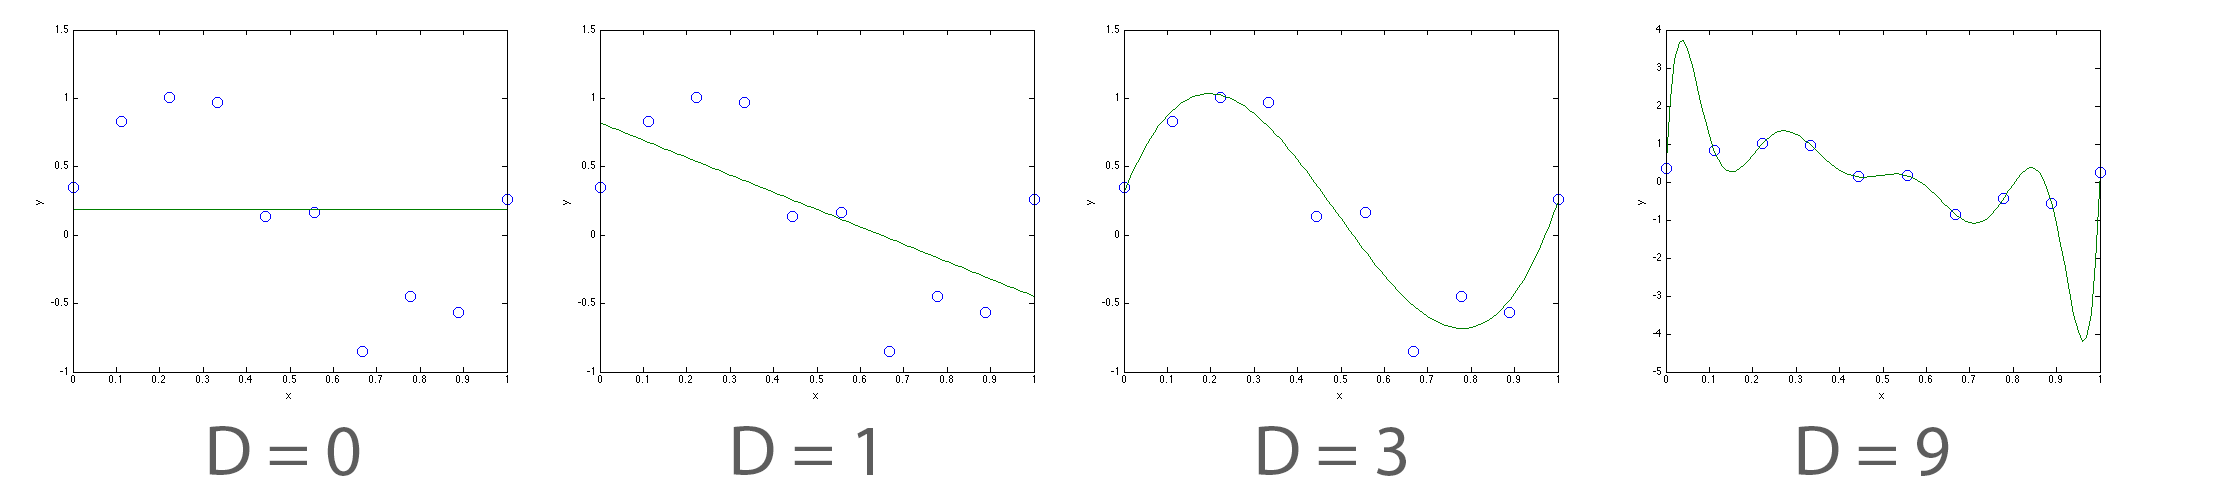
\includegraphics[width=1.0\textwidth]{figures/problem_2_1_full.png}
\end{figure}

\subsection{Gradient Descent}
The other approach is to optimize $W$ by gradient descent. We use the derivative of the error function in order to find a local minimum that satisfies a convergence threshold. For this data set, we use the \textbf{$\overrightarrow{0}$} vector as our initial guess. We use a step size of 0.01 as a parameter to gradient descent. Smaller step sizes take too long to converge and do not improve the final result, while larger step sizes ($> 0.1$) will sometimes never find a solution. A convergence threshold of $10^{-6}$ seems to work well, and it takes around $200$ iterations for the gradient descent algorithm to converge. \\
\\
\indent As expected, the gradient descent method takes significantly longer to run than the analytic solution. The gradient descent method is anywhere from 3 times as slow to 100 times as slow as the exact solution. \textbf{XXX add comparison to matlab optimizers} \\
\\
\begin{figure}[h!]\label{fig-gradient}
  \caption{Gradient descent solution for the linear regress problem with an initial guess of \textbf{0}, a step size of 0.01 and a convergence threshold of $10^{-6}$.}
  \centering
    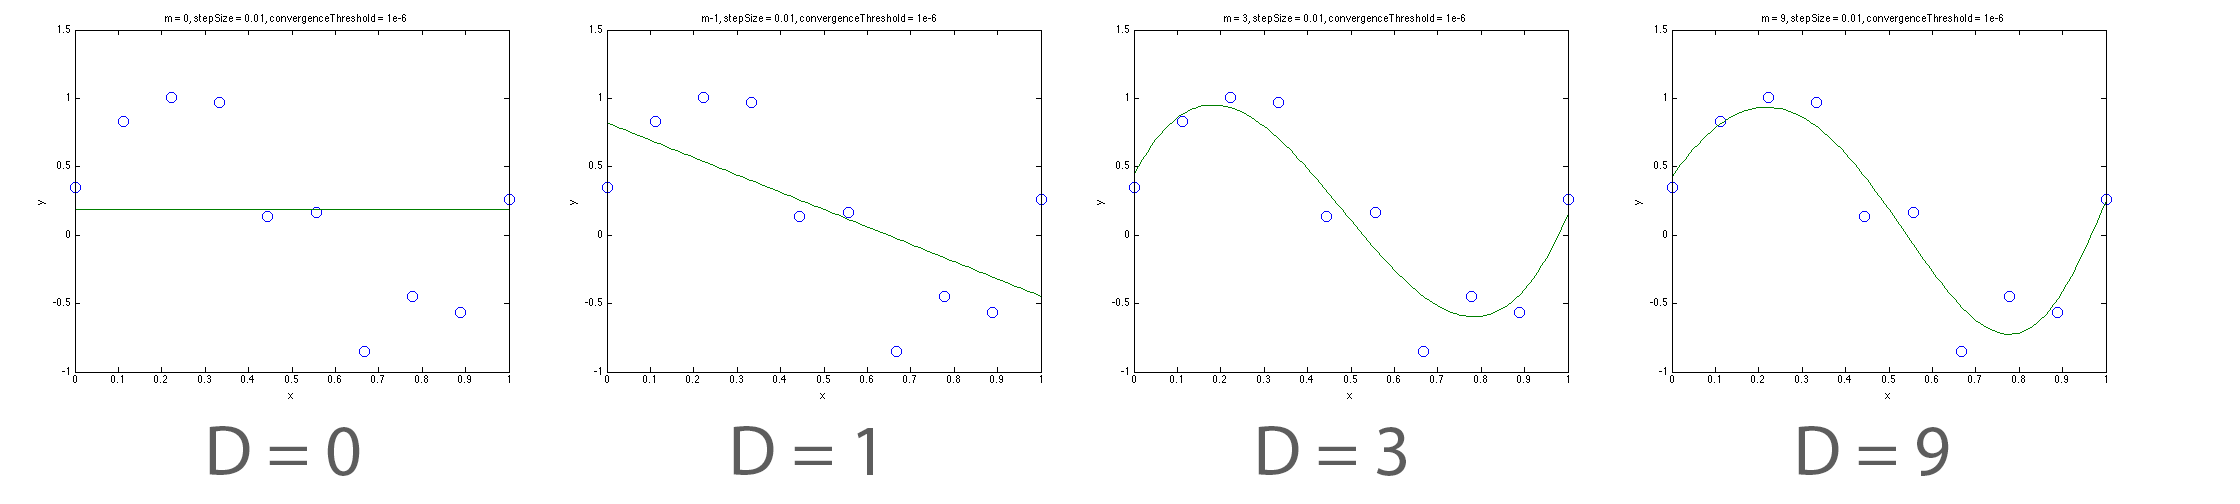
\includegraphics[width=1.0\textwidth]{figures/problem_2_2_full.png}
\end{figure}

\indent Figure~\ref{fig-gradient} shows the results of the gradient descent algorithm with our chosen parameters. The resulting $W$ vector produces a similar curve as the analytic solution for small values of $D$ but starts to diverge from the optimal $W$ as $D$ grows larger. Whereas the analytic solution for $D=9$ fits strongly to the data, the gradient descent solution does not manage to find the global optimum. It is likely that the gradient descent solution gets stuck in a local minimum that is not as optimal as the analytic solution.

\section{Ridge Regression}\label{sec-ridge}

In order to avoid over-fitting, we introduce a parameter $\lambda$ which governs the bias/variance trade-off. Larger values of $\lambda$ introduce bias and reduce variance by decreasing the norm of the weight vector. Another way to view ridge regression is to observe that we are minimizing the same error function with a constraint on the norm of the weight vector. \\
\\
\indent Solving analytically in the same way as Equation~\ref{eq-analytic}, the solution for the weight vector which minimizes error becomes:
\begin{equation}
W_{ridge} = (\textbf{Z}^\textnormal{T}\textbf{Z}+\lambda \textbf{I})^{-1} \textbf{Z}^\textnormal{T} Y_c,
\end{equation}
where $\textbf{Z}$ is a "centered" data matrix ($z_j^{(i)} = x_j^{(i)} - \bar{x}_j$), and $Y_c$ is a "centered" version of $Y$ where the mean of all values is 0. \\
\\
\indent

\subsection{Implementation}

\begin{figure}[h!]\label{fig-ridge-bishop}
  \caption{Bishop data set with various feature sets and lambda values.}
  \centering
    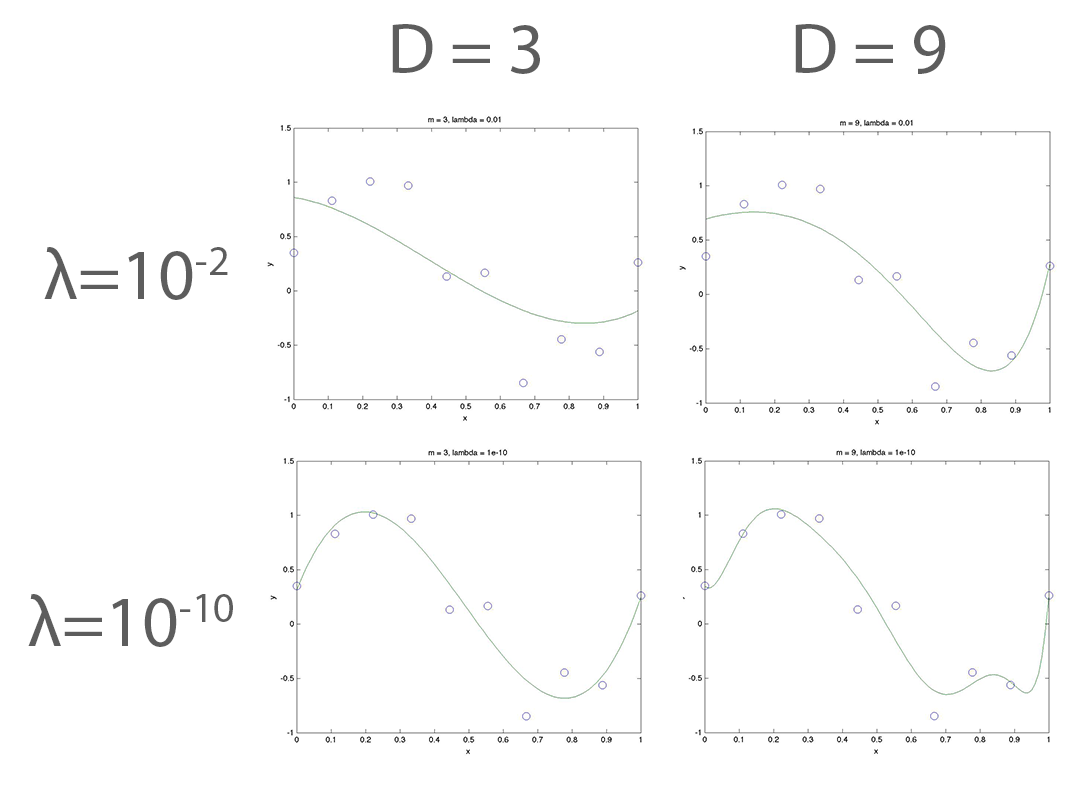
\includegraphics[width=0.5\textwidth]{figures/problem_2_3_bishop.png}
\end{figure}

Ridge regression was implemented and tested on the same data set as in Section~\ref{sec-basis}. Figure~\ref{fig-ridge-bishop} shows the results for various feature sets and lambda values. Higher values of lambda prevented over-fitting but also increased the observed sum-squared error. For $D = 9$ introducing the $\lambda$ parameter definitely improved the solution.

\subsection{Model Selection}

\subsection{Real World Data}
\end{document}
